
\begin{figure}[tbhp]
        \centering
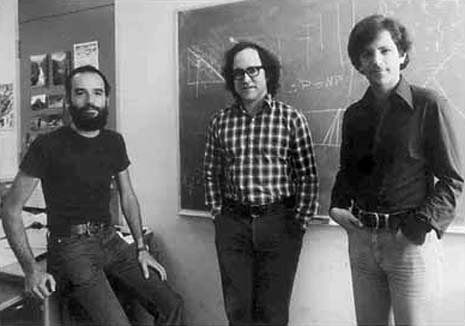
\includegraphics[width=0.75\textwidth]{./images/rsa.jpeg}
        \caption{Adi Shamir, Ronald Rivest, and Leonard Adelman}\label{fig:rsa}
\end{figure}

\section{Schmidt-Samoa (SS) Algorithm}
\epigraphwidth=0.4\textwidth
\epigraph{\emph{The magic words are \emph{Squeamish Ossifrage}.}}{---Ronald L. Rivest}

\noindent
The security of RSA relies on the practical difficulty of
factoring the product of two large prime numbers, known as the
\emph{factoring problem}. However, doing so would allow an adversary
to factor \emph{all} ciphertexts encrypted under that key.
Decrypting particular RSA ciphertexts is known as the \emph{RSA problem}.
At first look it would appear that the RSA problem may be easier than factoring,
and there are some cryptographers who believe this is the case.
Though there are no published, efficient methods to break RSA if a large enough key
is used -- short of building a \emph{quantum computer} and running Shor's algorithm on it --
this theoretical gap between the factoring problem and the RSA problem is not ideal.
The Schmidt-Samoa algorithm rectifies this theoretical problem,
by modifying the RSA algorithm in such a way that the SS problem is \emph{provably equivalent}
to the factoring problem. However, this property comes as the cost of efficiency,
which is why today's cryptographic protocols have largely ignored SS in favor of RSA.

SS involves a public key and a private key. Everyone can know the
public key, and it is used for encrypting messages. The intention is
that messages encrypted with the public key can only be decrypted by
using the private key.

The public key consists of the modulus $n$, which is composed of two large, random primes $p$ and $q$.
The private key consists of the private exponent $d$ and the private modulus $\lcm(p - 1, q - 1)$,
which must be kept
secret; $p$, $q$ must also be kept secret since they
are used to calculate $d$ and $\lcm(p - 1, q - 1)$.
In fact, $p$ and $q$ can be discarded after $d$
has been computed.

We proceed by choosing two large random primes $p$ and $q$, these
numbers must be kept secret. In particular we want large random primes,
where $p \nmid q - 1$ and $q \nmid p - 1$ and both $p - 1$ and $q - 1$ have
large prime factors. We then publish the number $n = p^2 q$. You
might wonder why we can do this, and the reason is that it is
\emph{believed} to be hard to factor large composite integers into their
constituent primes. The \emph{fundamental theorem of arithmetic} tells
us that every integer has a \emph{unique} prime factorization.

We now calculate $\lcm(p - 1, q - 1)$, the private modulus,
and a unique secret integer $d\in \{0, \ldots, n-1\}$ such
that $d \times n \equiv 1 \pmod{\lcm(p - 1, q - 1)}$. How do we find this $d$?
It turns out that we have known how to do it for more than $2300$
years---we use an algorithm attributed to \emph{Euclid}. How is it that
we can easily calculate $d$ while our adversary cannot? We know a secret
that he does not: we know $p$ and $q$ while he only knows $n$. We call
$d$ our private exponent.
Together $pq$ and $d$ make up our \emph{private key}.

We now define two functions: $E(m) = m^n \pmod{n}$ and $D(c) = c^d
\pmod{pq}$. We will show in \S\ref{proof} that $\forall m \in \{0,
\ldots, pq - 1\}$ that $D(E(m)) = m$.

There's a catch here.
Say we want to publish the public key, so that people can encrypt messages for us.
We know that our message space is $\{0, \ldots, pq - 1\}$,
and that messages outside of that space will not decrypt correctly,
so along with $n$ we have to publish $pq$, right? {\em Wrong!}
If we did that, then anyone could calculate $p = n / pq$ and $q = pq / p$.
With that information anyone can determine our private key!
Instead, we observe that
\begin{align*}
    \sqrt{n} = & p\sqrt{q} \\
             < pq,
\end{align*}
so instead of using our full message space, $\{0, ..., pq - 1\}$,
we will just allow messages in a truncated message space $\{0, \sqrt{n} - 1\}$.

How do we know that this doesn't break our security like we would have had we published $pq$?
Because, we are just computing some function of the public information $n$.
For a system to be secure, it must be able to keep the private key secret against adversaries
with polynomial resources and access to $n$. Because Schmidt-Samoa is secure, asking people
to compute a polynomial time algorithm with $n$ as the input can't give the adversary any advantage
that he didn't already have!

This issue highlights something important: don't write your own cryptographic algorithms! (this assignment excluded)
It's very easy to make mistakes and write algorithms that look secure but are trivial to break.
As Bruce Schneier said, "anyone, from the most clueless amateur to the best cryptographer,
can create an algorithm that he himself can't break."
